\section{Division into objects}

To assure real modularity of our template, more divisions were proposed than only the one mentioned at the beginning of this chapter; their structure being represented in Figure \ref{objectStructure}.

We already mentioned the separation of the Algorithm from the State Space. It is useful to think of the Algorithm as of a decision-maker. Its role is restricted to making decisions on acceptance or rejections of the proposals generated by the State Space and then on ordering the State Space to perform all the subsequent actions. The information on which the Algorithm bases its decisions depends on the points from the State Space only indirectly, via the evaluations of densities ( or, in the discrete case -- probability functions ) at the proposal points. A third candidate for an entity thus appears - namely an object whose methods would serve to measure some characteristic of the State Space sample points for the use in the decision-making of the Algorithm. We called this entity the Target Measure. 

The very idea behind the Target Measure entity is that it should serve as a container for user-defined probability function or a density together with every additional data-structure required for its evaluation. Moreover, in case the user was interested in testing the \PT's potential on some toy-example, that was analytically tractable or could be simulated using any other simpler and more efficient technique, the Target Measure entity would be the place to store any additional methods tied with this particular distribution. For example, in our simulations (confront Chapter \ref{simulationsAndResults}) we could  additionally provide efficient methods for quantile simulations and evaluates of the real distribuant. Implementations of these functions were collected as methods of the appropriately named instatiation of the Target Measure structure.  

\begin{figure}
	\centering 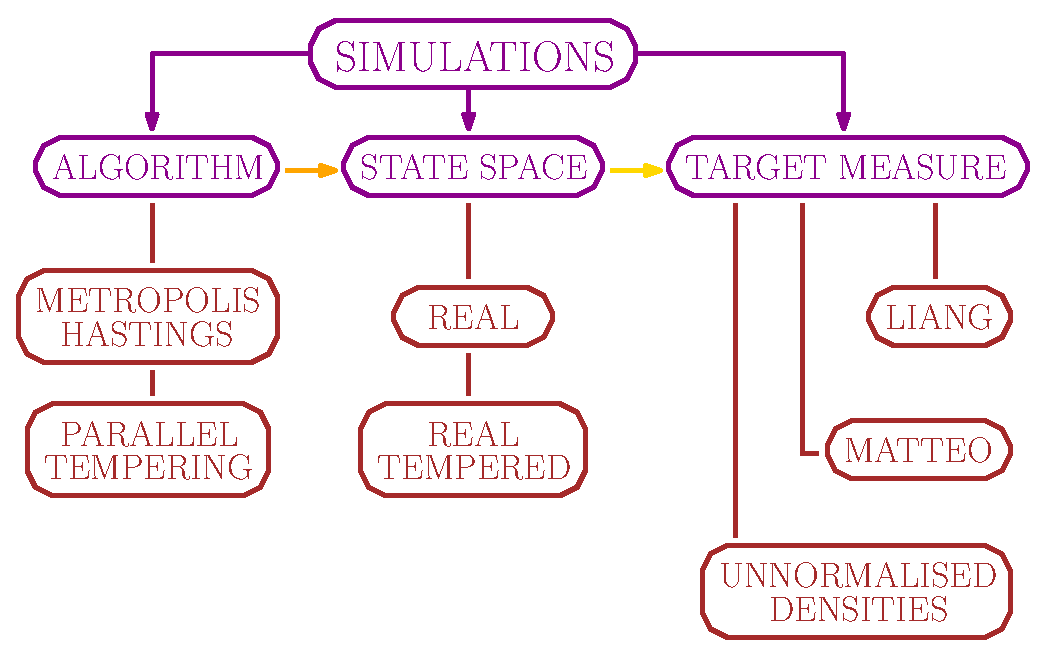
\includegraphics[keepaspectratio=true, width =\linewidth]{./img/objectStructure.eps}
	\caption{Current operational entity-relations diagram.}\label{objectStructure}
\end{figure}

The reason for separating the Target Measure from the State Space is again dictated by the modularity requirement. Totally different models can be modelled on the same State Space, the only difference being the way the probability is assigned. It is therefore natural to define an entity whose task will be to serve as a warehouse for sample points, together with efficient methods or reading them, and in the end -- presenting the results to the user. These things, to some extent, can be done for any probability measure defined by the user. 

The Object Oriented paradigm gives the programmer the tool of inheritance. Its role is to assure no code copying when several programmes share the same structure and differ only at some minor implementation details. In this implementation we have noticed that the \PT, being an extension to the \MH, differs only in the appearance of the swap stage and its methods, the Random Walk stage being almost the same\footnote{The difference being that it is called for several chains instead of one.}.    

All the entities must be linked, so that different parts of programme could call methods of other entities. Because of certain Reference Classes limititions\footnote{As pointed out before, Reference Classes are relatively new, and, as such, poorly documented. With trial and error it has been checked, that this particular choice of entity-nesting simply works.}, the Algrorithm has a pointer on the State Space, which in its turn has a pointer on the Target Measure. These relationships are visualised in Figure \ref{objectStructure} under the form of golden arrows. Under different circumstances, different realisations of objects will appear as the Algorithm, the State Space, and the Target Measure. For instantance, if the user wanted to carry out standard Metropolis-Hastings calculations on the three-dimensional euclidean space and check how it copes with the density function he provided, then the programme would have to initialise first the Unnormalised Density as the realisation of the Target Measure entity. Then, initialise the Real space as an instatiation of the State Space and set the pointer for the previously initialised. Finally, it would initialise the Metropolis-Hastings as the operational Algorithm and set the pointer on the previously initialised State Space, being the Real space. To automate this chain of initialisations, a controller entity was established under the name of Simulation ( see Figure \ref{objectStructure} ). Two additional functions were written, \textsc{Metro} and \textsc{PT}, serving as wrappers to the more general Reference Class constructor of the Simulation object. 

Continuing on the example, the user would simply had to call

\begin{lstlisting}
	Example <- Metro(
		n = 1000,
		space = 'real',
		spaceDim = 2,
		targetDensity = userDefinedDensity
	)
\end{lstlisting}  
where \textsc{userDefinedDensity} is an R-implemented unnormalised density function\footnote{In future versions \Cpp\, calls will be usable.}.  

The presented object structure is far from final. Hopefully it will evolve in time, trying to match the needs of various users. We already plan the separation of the swap distributions from the Parallel Tempering entity, giving the user the possibility to check his own swapping strategies, possibly better suited for their needs.